\documentclass[10.5pt,a4paper]{article}
\usepackage[a4paper,margin=1.7cm,top=1.4cm,bottom=1.5cm]{geometry}
\usepackage[T1]{fontenc}
\usepackage{lmodern}
\usepackage{microtype}
\usepackage{graphicx}
\usepackage{booktabs}
\usepackage{enumitem}
\usepackage{xcolor}
\usepackage[hidelinks]{hyperref}
\usepackage{titlesec}
\setlist{nosep,leftmargin=1.2em}
\titleformat{\section}{\normalsize\bfseries}{\thesection.}{0.5em}{}
\titlespacing*{\section}{0pt}{7pt}{3pt}
\setlength{\parindent}{0pt}
\setlength{\parskip}{4pt}
\newcommand{\code}[1]{\texttt{#1}}
\definecolor{grey}{HTML}{52514E}

\begin{document}

{\large\bfseries Pressure-driven flow of the viscoelastic Oldroyd-B fluid in narrow non-uniform geometries: re-solved with a physics-informed neural network}\\[3pt]
{\small Rahul Arvind Masand (2022CH71476) \quad·\quad CLL731 term paper (ML) \quad·\quad IIT Delhi \quad·\quad November 2026}\\[1pt]
{\small Code, results and report: \url{https://github.com/RM1102/CLL731-OldroydB-PINN}}

\vspace{-2pt}\noindent\rule{\linewidth}{0.4pt}

\section{Purpose}
Honey flows smoothly; honey with long polymer molecules dissolved in it behaves as if it were full of tiny rubber bands. When such a liquid is squeezed through a narrowing channel, the molecules are stretched and pull back. Boyko \& Stone (\emph{J.\ Fluid Mech.}\ 936, A23, 2022) asked how this elasticity changes the pressure needed to push a fixed flow rate through a narrow channel that contracts 4:1. They used the Oldroyd-B model and gave formulas valid for weak elasticity (small Deborah number De), checked against computer simulations. Their answer: elasticity \emph{lowers} the pressure drop.

\textbf{Aim of this project:} solve the same equations with a \emph{physics-informed neural network} (PINN), a network trained only to satisfy the flow equations, never shown a solution, and check it carefully against the paper.

\section{What was done}
\begin{enumerate}[label=\arabic*.]
\item \textbf{Checked the paper.} Re-derived its whole low-De solution with symbolic algebra (SymPy). Every formula is confirmed except one sign typo in arXiv eq.\ (3.16b).
\item \textbf{Recovered the paper's simulation data.} The data were not published, but the figures in the PDF are vector drawings, so the exact data points were read out of the file.
\item \textbf{Built an independent reference solver} for the narrow-channel limit. It agrees with the paper's simulations within 0.37\,\%. A finding on the way: solving station by station down the channel fails for any De $>0$, because the stretched molecules and the velocity affect each other in both directions. The whole channel must be solved at once, which a PINN does naturally.
\item \textbf{Designed the PINN} so that every boundary condition holds exactly by construction (a stream function for the velocity, symmetric inputs, exact inflow stress). The training loss then contains only the equations. Splitting the pressure into a part along the channel and a small part across it removed a hidden 0.25\,\% bias.
\item \textbf{Trained 16 networks plus one network that takes De as an input}, on a laptop (CPU and its GPU), for the narrow-channel limit and for the paper's two real channels ($\epsilon = 0.02$ and $0.1$), at De from 0 to 0.3.
\end{enumerate}

\section{Main results}
\begin{center}\small
\begin{tabular}{@{}lll@{}}
\toprule
Check & Result & Reference\\
\midrule
PINN, narrow-channel limit, De $\le 0.3$ & within 0.22\,\% & our reference solver\\
PINN, full 2-D, both of the paper's channels & within 0.68\,\% & the paper's simulations\\
Paper's 3rd-order formula at De $=0.3$ & 23--26\,\% too low & the paper's simulations\\
PINN stress fields & 0.01--0.5\,\% over most of the channel & our reference solver\\
\bottomrule
\end{tabular}
\end{center}
\vspace{-4pt}
\begin{center}
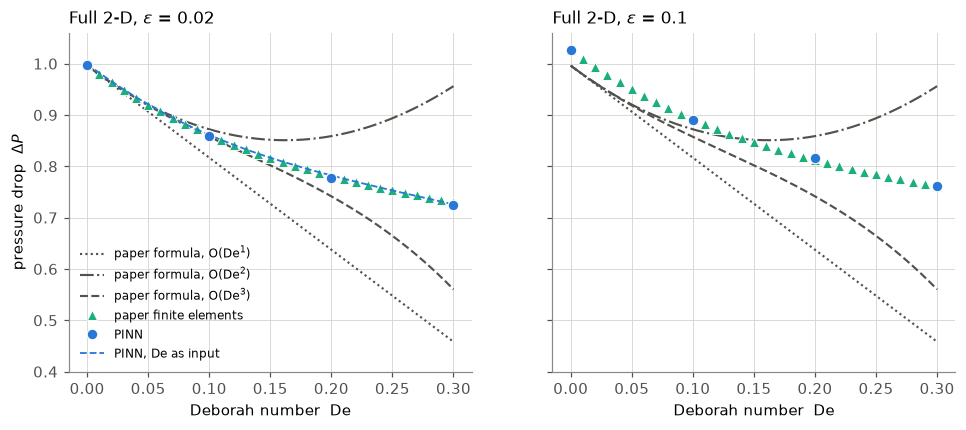
\includegraphics[width=0.86\linewidth]{../04_results/figures/fig08_pinn_circles_against_the_papers.png}\\[-1pt]
{\footnotesize\color{grey} Pressure drop against De for the paper's two channels. Circles: PINN. Triangles: the paper's simulations. Lines: the paper's formulas.}
\end{center}
The PINN follows the simulations over the whole range, including De $=0.2$--$0.3$ where the formula fails. The pressure drop falls because of the gradient of the polymer \emph{shear} stress, as the paper says. Errors are largest (a few percent) at the two corners where the wall slope changes suddenly.

\section{How to run it (Windows or Mac)}
Install Python 3.10--3.13 from python.org (on Windows tick ``Add python.exe to PATH''). Then, in a terminal:\\[2pt]
\begin{tabular}{@{}ll@{}}
Windows: & \code{git clone https://github.com/RM1102/CLL731-OldroydB-PINN.git}\\
 & \code{cd CLL731-OldroydB-PINN} \quad then \quad \code{setup\_and\_run.bat}\\
Mac: & same two lines, then \quad \code{bash setup\_and\_run.sh}\\
\end{tabular}\\[2pt]
Without git: on the GitHub page click \emph{Code $\rightarrow$ Download ZIP}, unzip, and double-click \code{setup\_and\_run.bat} (Windows) or \code{setup\_and\_run\_mac.command} (Mac). The script sets up a private Python environment inside the folder and shows a menu:
\begin{enumerate}[label=\arabic*)]
\item \textbf{explorer window}: pick a channel and a field, move the De slider, type a point to read the predicted values;
\item \textbf{notebook}: the full report with code and charts (runs in about 20 s using the saved networks);
\item \textbf{quick check} (about 10 s);
\item \textbf{retrain everything}.
\end{enumerate}
\textbf{Time warnings.} The first setup downloads about 1\,GB and takes 5--15 minutes. Retraining takes about \textbf{4 hours} on a laptop and is not needed: all trained networks are included. To read the report without installing anything, open \code{05\_notebook/CLL731\_OldroydB\_PINN.html} in a browser.

\section{Using the trained PINN for predictions}
A trained PINN is a formula: given a position and De, it returns velocity, pressure and polymer stress in a fraction of a second, without solving anything again. Besides the explorer window, \code{predict.py} answers from the command line, for example \code{python predict.py -{}-case eps0.02 -{}-De 0.2 -{}-dp} for the pressure drop (also in pascals for the paper's channel), \code{-{}-point 0.5 0.3} for every field at a point, or \code{-{}-csv out.csv} for a whole field. Valid range: the paper's channel ($\alpha=4$, $\tilde\beta=0.4$) and $0 \le \mathrm{De} \le 0.3$.

\section{Limits and acknowledgement}
The PINN takes minutes to train per case, where our reference solver takes seconds; its strengths are exact boundary conditions, no mesh, and one network that answers any De instantly. Accuracy is limited at the two corners. Higher De ($>0.5$), where Oldroyd-B stresses grow without bound, was not attempted.
\emph{Use of AI:} the literature search, code and text were developed with the help of an AI assistant (Claude), as stated in the project proposal; all results were checked against the paper and an independent solver.

\end{document}
